%!TEX root = ../main.tex
\chapter{Future $e^+e^-$ linear collider experiments}
\label{chap:FutureColliders}

Currently, the only high energy collider in operation is the \textit{Large Hadron Collider} (LHC) at CERN between Switzerland and France. The construction of the LHC started in 1995, was achieved in 2008 and its operation started in 2009. The LHC machine lies in a long underground tunnel of 27 km circumference and is colliding protons at a center-of-mass energy up to $\sqrt{s} = 14$ TeV using supra-conducting magnets. It is probing the Standard Model to an unprecedented energy scale and searches for unknown particles beyond the Standard Model. The discovery of the Higgs Boson in 2012 was one of the major milestones of the LHC. The colliding particles are protons which are composites particles, thus only a fraction of the energy is available during the collision. These collisions are very complex and make some measurements almost impossible at the LHC.

In the past, $e^+e^-$ colliders have been complementary tools to hadron colliders like the \textit{Large Electron-Positron Collider} (\acrshort{lep}) at \acrshort{cern} and Tevatron at Fermilab. A limitation of $e^+e^-$ ring colliders is the maximum achievable collision energy which is limited by the energy losses of the particles due to the synchrotron radiation. The synchrotron radiation power scales as
\begin{equation}
  P_{synchrotron} \propto \frac{E^4}{R \times m^4}
\end{equation}
with $E$ the particle energy, $m$ the mass of the particle and $R$ the accelerator radius. The mass dependence makes the radiation losses significantly higher than protons. The maximum energy achieved by a $e^+e^-$ ring collider was of around a center-of-mass energy of $\sqrt{s} = 210$ GeV with the LEP. In this conditions, around 8 MW of energy is lost by synchrotron radiation.
Therefore, it is most likely that the next $e^+e^-$ collider will be a linear accelerator to achieve energies near the TeV scale.

The \textit{International Linear Collider} (\acrshort{ilc}) and The \textit{Compact Linear Collider} (\acrshort{clic}) are two proposed particle physics accelerator complementary to the LHC. The ILC is designed to collide electrons and positrons at a center-of-mass energy between 250 GeV to 500 GeV with a possible upgrade to 1 TeV. The advantage of the ILC is that it provides a reduced background and cleaner events compared to a hadron collider thus allowing for high precision measurements. The following section will give a short summary of the ILC machine and its detectors and based on the ILC Technical Design Report (TDR) \cite{ILC_TDR_Vol1, ILC_TDR_Vol2, ILC_TDR_Vol3.1, ILC_TDR_Vol3.2, ILC_TDR_Vol4}.

\section{The International Linear Collider (ILC)}
\label{sec:ILC}

The International Linear Collider (ILC) is a planned 31 km long $e^+e^-$ linear collider to be built in Japan with a design peak luminosity of around $2 \times 10^{34} cm^{-2}s^{-1}$ and a center-of-mass energy of 500 GeV. An upgrade up to 1 TeV center-of-mass energy and a higher luminosity is possible. Polarization up to 80\% for electrons and 30\% for positrons can be achieved enabling the enhancement of rates and the reduction of SM background. The polarization is a crucial ingredient in the ILC program. It uses supra-conducting RF (SCRF) cavities to accelerate electrons and positrons. The project is currently under discussion between the governments and a decision by the end of 2018 should be reached. A schematic of the ILC layout is shown in figure \ref{fig:ILC_schematic}.

\begin{figure}[htbp!]
  \centering
  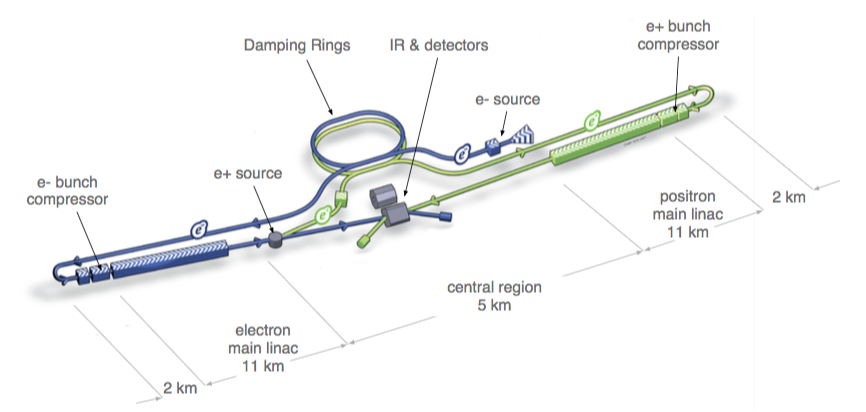
\includegraphics[width=0.7\linewidth]{chap2/fig/ILC_schematic.png}
  \caption{Schematic of the International Linear Collider (not to scale). Taken from \cite{ILC_TDR_Vol1}.} \label{fig:ILC_schematic}
\end{figure}

The electron beam is produced by a laser illuminating a photocathode of GaAs in a DC gun. It provides the bunches of electrons with a polarization of 90\%. The bunches are accelerated to 5 GeV in a \acrshort{scrf} booster before being collected in the dumping ring. The dumping ring has a circumference of 3.2 km where bunch trains are formed and the emittance of the beam reduced by 5 orders of magnitude to 20 nm. It is achieved by the succession of normal magnets, supra-conducting magnets and wiggler magnets. The wiggler magnets cool the beam by dumping synchrotron radiation thus reducing the beam emittance. The bunch trains formed by the ring are around 200 ms apart containing more than 1000 electron bunches.

The electron beam is then transported by the Ring to Main Linac (RTML), accelerating electrons from 5 GeV to 15 GeV while compressing the bunch-length to few micrometers required by the integration region (IR).

The main linac of the ILC accelerates the electron beam up to 250 GeV by using supra-conductive RF cavities of niobium operated at 2 Kelvins housed in cryomodules. The RF power is delivered by a system of Klystrons. The average gradient of the cavities is around 31.5 $\frac{MV}{m}$ with a quality factor $Q_0 \geqslant 10^{10}$. The synchrotron sources of FLASH and recently of the European X-Ray Free Electron Laser (XFEL) based at DESY, are a demonstration of the mass-production and operation of cryomodules which represents around 1\% of the ILC.

After the acceleration, the electron beam is transported through a supra-conducting helical undulator which generates photons between 10 to 30 MeV. Then the electron beam is separated from the photon beam and transported by the Beam Delivery System (\acrshort{bds}) to the IR. The BDS focuses the beam down to 474 nm $\times$ 5.9 nm (x and y respectively at $\sqrt{s} = 500$ GeV) to reach the luminosity goal of $2 \times 10^{34} cm^{-2}s^{-1}$.

The photons are directed onto a thin ($0.4 X_0$) titanium alloy (Ti) target producing elec\-tron\--positron pairs. The positrons are accelerated to 400 MeV in a first step while the remaining electrons and photons are dumped. The positrons are accelerated to 5 GeV by a booster and injected into a dumping ring, parallel to the electron ring. From there, the positron beam follows a similar beam line as the electron beam and both beams are brought into collision at the IR, where two detectors lie that can be operated in a push-pull configuration.

\begin{figure}[htbp!]
  \centering
  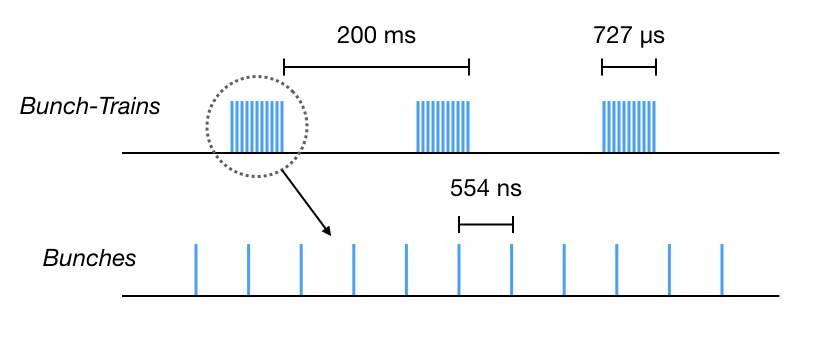
\includegraphics[width=0.7\linewidth]{chap2/fig/BeamStructure.jpeg}
  \caption{Schematic of beam structure of the ILC operated a design parameters.} \label{fig:ILC_BeamStruct}
\end{figure}

The beam structure of the ILC consists of bunch-trains of 1312 bunches of $2 \times 10^{10}$ particles each and separated by around 550 ns. The distance between bunch-trains is around 200 ms corresponding to a 5 Hz repetition frequency (up to 10 Hz depending on the running scenario). A schematic of the beam structure is shown in figure \ref{fig:ILC_BeamStruct}.

The CLIC concept \cite{CLIC_CDR} is drastically different in the design and technology used. CLIC uses normal conducting copper cavities operated at 12 GHz much higher than ILC (1.3 GHz). It uses a two-beam operation scheme where a high current, low energy drive beam provides RF power to accelerate a low current, high energy beam. By this mean, a center-of-mass energy up to $\sqrt{s} = 3$ TeV could be achieved. The CLIC technology is yet not mature compared to the ILC and still needs several years of R\&D before a full CLIC accelerator could be constructed.

\section{The International Large Detector (ILD)}
\label{sec:ILD}

The physics program of the ILC is quite ambitious. In order to realize it, significant advances in detector performance are essential. The detector concepts for the ILC are focused on the \textit{Particle Flow} approach. The Particle Flow approach is discussed in section \ref{sec:PFA}. It is aiming to reconstruct individually each particle in an event. This requires an unprecedented spatial resolution in all sub-detectors to efficiently separate charged and neutral particles even within jets. This motivates for a highly efficient tracking system and highly granular calorimeters but also a sophisticated reconstruction software.

At the ILC, it is planned to have two detector experiments sharing the interaction region in a push-pull configuration. One detector occupies the IR while the other detector is parked in the detector hall. Both detectors can be moved in and out of the IR periodically every few weeks. Two detector concepts have been developed in the ILC Technical Design Report \cite{ILC_TDR_Vol4}, the \textit{Silicon Detector} (\acrshort{sid}) and the \textit{International Large Detector} (\acrshort{ild}). A detailed detector simulation is available for both of the concepts and has been used extensively in the study of the potential of ILC physics as well as detector optimizations. The detectors concepts contain realistic implementations of all sub-detectors and have been cross-checked with prototype data if possible (see chapter \ref{chap:CALICE_Det}). In the following, the ILD detector will be briefly described.

The ILD detector is a multi-purpose detector. The tracking system and the calorimeter systems are both located within a supra-conducting solenoid magnet of 3.4 m radius providing a field of 3.5 T parallel to the beam axis. Schematics of the ILD detector can be seen in figure \ref{fig:ILD}.

\begin{figure}[htbp!]
  \centering
  \begin{subfigure}[t]{0.49\textwidth}
    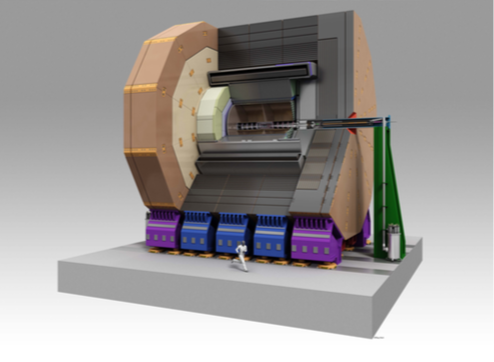
\includegraphics[width=1.\linewidth]{chap2/fig/ILD_full.png}
  \end{subfigure}
  \hfill
  \begin{subfigure}[t]{0.49\textwidth}
    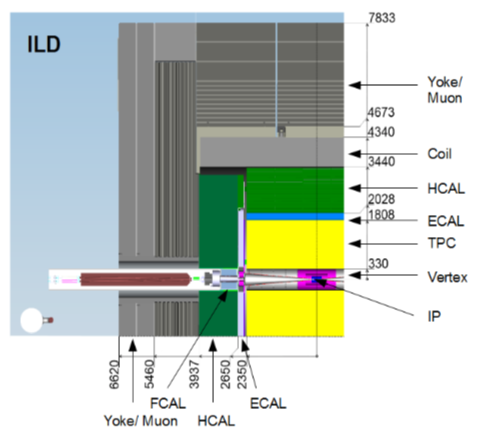
\includegraphics[width=1.\linewidth]{chap2/fig/ILD_layout.png}
  \end{subfigure}
  \caption{Schematic views of the ILD detector. Dimensions on the right figure are in mm. \cite{ILC_TDR_Vol4}.} \label{fig:ILD}
\end{figure}

\subsection{ILD Tracking System}

The ILD Tracking system consists of a multi-layer pixel vertex detector (\acrshort{vtx}) at the innermost part, at around 1.6 cm of the beam pipe. Different geometries are proposed, a three double layer or a five single layer silicon pixel geometry. Additionally, two layers of silicon strip detector (\acrshort{sit}) are placed around the vertex detector to close the gap between the VTX and the \textit{Time Projection Chamber} (\acrshort{tpc}). In the forward region, silicon pixel disks and silicon strip disks (\acrshort{ftd}) are installed to provide coverage at track low angles. The VTX offers position hit resolutions of less than \SI{6}{\micro\meter} with a very low material budget of 0.15\% $X_0$ per layer. The SIT and FTD pixel detectors offer similar position hit resolutions with a material budget of 0.65\% $X_0$. While the technology has not been decided yet, the VTX is optimized for the higher single point resolution and minimum material budget. The high resolution of the VTX offers the best performance for the flavor tagging of jets, even in the very forward direction.

The main feature of the ILD tracking system is a large TPC providing more than 200 points per track, covering from 330 mm to 1808 mm in radius. The TPC uses the fact that a particle traversing the gas inside the TPC, ionize it along its trajectory. The free electrons are then drifting towards the endcaps (endplates) by an electric field parallel to the beam axis. The endplate detects the ionization electrons by a \textit{Gas Electron Multiplier} (\acrshort{gem}) or a \textit{Micro-Mesh Gaseous Structure} (\acrshort{micromegas}) readout system. The spatial resolution of the TPC is better than \SI{100}{\micro\meter} and also offer a double hit resolution in the order of less than 2 mm. This resolution is worse than silicon tracking can offer but the TPC presents the advantage of a very low material budget, continuous tracking and excellent reconstruction of the non-pointing tracks (Kinks) from multiple scattering. In addition, the TPC offers the possibility of particle identification via the specific energy loss $\frac{dE}{dx}$ (see subsection \ref{sec:PartInter}).

A combined momentum resolution of $\sigma_{1/p_T} = 2 \times 10^{-5}$ GeV$^{-1}$ has been achieved for high momenta for the ILD tracking system.

\subsection{ILD Calorimeter System}

The ILD calorimeter system is designed and optimized for \textit{Particle Flow} (see section \ref{sec:PFA}). It is aiming to achieve a jet energy resolution $\sigma_E/E$ of around 3-4 \% for the energy range of 45 to 250 GeV. The excellent track reconstruction combined with the calorimeter system requires an unprecedented 3D granularity for the calorimeters to achieve such goals. To minimize material and optimize track associations to depositions in the calorimeters, they are located inside the solenoid magnet thus limiting the depth of the calorimeters. A reasonable trade-off between intrinsic energy resolution and granularity is present in the ILD calorimeter system.

The ILD baseline consists of the electromagnetic calorimeter (\acrshort{ecal}) using silicon-bas\-ed readout with a $5 \times 5$ mm segmentation in a tungsten absorber, allowing a very compact design and the hadronic calorimeter with scintillator-tile based analog readout (\acrshort{ahcal}) with a segmentation of $3 \times 3$ cm in a steel absorber. More details on the AHCAL can be read in chapter \ref{chap:CALICE_Det}. In the forward region, additional calorimeters are placed, LumiCal, BeamCal and LHCAL for luminosity monitoring, beamstralhung measurement and hermiticity at low angles.

After the solenoid magnet, an iron yoke returns the magnetic field and is planned to be instrumented with scintillator strips or resistive plate chambers (\acrshort{rpc}) to serve as a muon detector and tail catcher for high energy jets.

\section{The SiD Detector}

The SiD detector concept is very similar to the ILD detector. It differs by its size much smaller than ILD, the use of a stronger magnetic field (5 T) and a full silicon tracking system instead of a TPC. The ECAL is the same using silicon as active material. Resistive plate chambers (RPCs) with gas as active material were planned to be used for the hadron calorimeter system but a recent change in the baseline design includes now a scintillator-tile hadronic calorimeter. The performance of SiD is very close in numbers to ILD.

\section{ILC Physics}
\label{sec:ILC_Physics}

The ILC Physics program is very ambitious and complementary to studies done at the LHC. The recent discovery of the Higgs Boson in the 125 GeV range at the LHC which was for several decades the missing block of the SM can be studied with much more precision with the ILC. The probing of the characteristics of the Higgs Boson to a percent level is necessary to validate the current SM but also to be able to observe any deviations to predictions that would be a strong hint for physics beyond the SM. Many other opportunities are provided by the ILC for the study of new physics, the Z and W Bosons and the top quark that can be studied with high precision. This section will describe few key points of the ILC physics program.

\subsection{Higgs Physics}

The ILC experiment provides a precise and model-independent measurement of the Higgs Boson characteristics such as its mass, full decay width and absolute coupling to SM particles. The precision on some of these parameters at LHC is significantly worse than for ILC where a clean, low background environment and well defined initial state is present. The full decay width is not accessible at the LHC in a model independent way thus absolute couplings also.

\subsubsection{Higgs production and decay modes}

There are two main production modes of the Higgs at the ILC, the \textit{Higgsstrahlung} and \textit{Vector Boson Fusion} (\acrshort{vbf}). The \textit{Higgsstrahlung} process is the production of a Higgs Boson in association with a Z Boson. For the VBF mode, either two Z or W Bosons fuse in a Higgs Boson in association with either an electron-positron pair or neutrino-antineutrino pair. The Feymann diagrams are shown in figure \ref{fig:HiggsProd}.

\begin{figure}[htbp!]
  \centering
  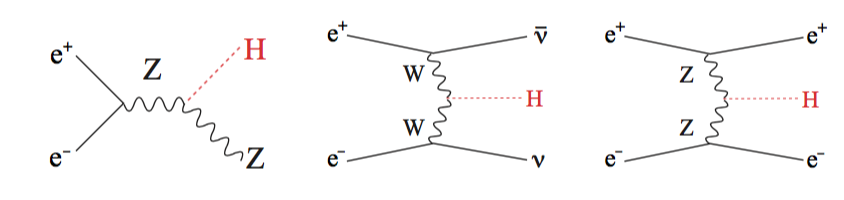
\includegraphics[width=1\linewidth]{chap2/fig/HiggsProd.png}
  \caption{Feymann diagrams for the Higgs production at the ILC at Tree level. \cite{ILC_TDR_Vol2}} \label{fig:HiggsProd}
\end{figure}

At $\sqrt{s}$ = 250 GeV, the Higgsstrahlung process is dominant, the production cross-section peaks at $\sqrt{s}$ = 250 GeV. At higher energies around $\sqrt{s}$ = 450 GeV, the VBF production cross-section starts to dominate. The figure \ref{fig:HiggsXS} shows the evolution of the Higgs production cross-section as function of center-of-mass energy $\sqrt{s}$.
The Higgs decays mostly into a pair of b quarks ($\sim$ 57\%). The next highest branching ratio (\acrshort{br}) is to a $WW^*$ pair ($\sim$ 21\%). Then in the order of few percents, the Higgs decays to $gg$, $ZZ^*$, $\tau \tau$, $cc$. The difference of BR between $h \rightarrow WW^*$ and $h \rightarrow ZZ^*$ is quite interesting with an order of magnitude difference. This explained by the fact that the one of the Z is further off-shell than the one of the W due to $m_h << 2 \times m_W < 2 \times m_Z$ thus suppressing the Z BR.
Other decays to $\mu \mu$, $\gamma \gamma$ and $Z\gamma$ are very rare below 1\%. Massless final states decays are possible through heavy quark loops (top loop). The main branching ratios are depicted in figure \ref{fig:HiggsBR}.

\begin{figure}[htbp!]
  \centering
  \begin{subfigure}[t]{0.49\textwidth}
    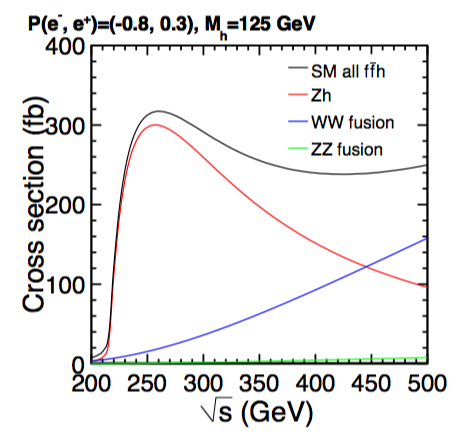
\includegraphics[width=1.\linewidth]{chap2/fig/HiggsXS.png}
    \caption{} \label{fig:HiggsXS}
  \end{subfigure}
  \hfill
  \begin{subfigure}[t]{0.49\textwidth}
    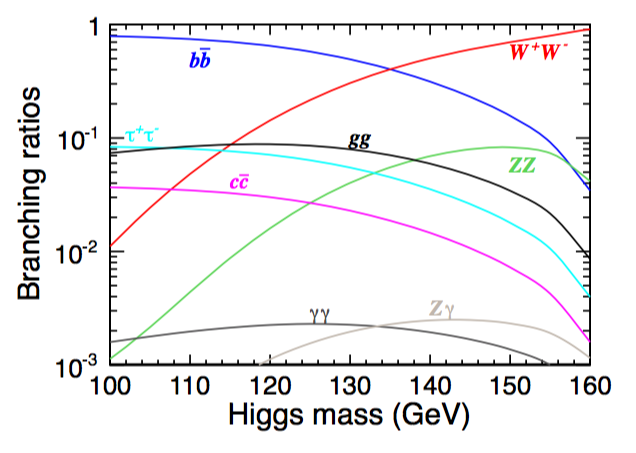
\includegraphics[width=1.\linewidth]{chap2/fig/HiggsBR.png}
    \caption{} \label{fig:HiggsBR}
  \end{subfigure}
  \caption{\subref{fig:HiggsXS}) Production cross-sections for the Higgs at the ILC as function of $\sqrt{s}$. \subref{fig:HiggsBR}) Higgs branching ratios as function of the Higgs mass.}
\end{figure}

\subsubsection{Recoil mass measurement}

At the ILC, the initial state of the collision is precisely known, offering a unique method to measure the Higgs mass. The recoil mass measurement, in the Higgsstrahlung process, aims at reconstructing the Z boson recoiling against the Higgs without the need to reconstruct the Higgs itself, no assumption is made on the decay mode. This enables a truly model-independent measurement of the Higgs mass and its full decay width with an unprecedented precision.

Events where the Z decays to a pair of charged leptons ($e^+e^-$ or $\mu^+ \mu^-$) are used and the recoil mass $m_{recoil}$ can be calculated as \cite{Yan:2016xyx}
\begin{equation}
  m_{recoil}^2 = (\sqrt{s} - (E_{l^+} + E_{l^-}))^2 -  |\textbf{p}_{l^+} + \textbf{p}_{l^-}|^2
\end{equation}
where $E_{l^j}$ and $\textbf{p}_{l^j}$ are the energy and momentum of the lepton pair from the Z decay. These events can be selected by constraining the invariant mass of the lepton pair to be consistent with the Z mass. A reconstructed recoil mass distribution for $Zh \rightarrow \mu^+\mu^-X$ is shown in figure \ref{fig:HiggsRecoilMuMu}.

\begin{figure}[htbp!]
  \centering
  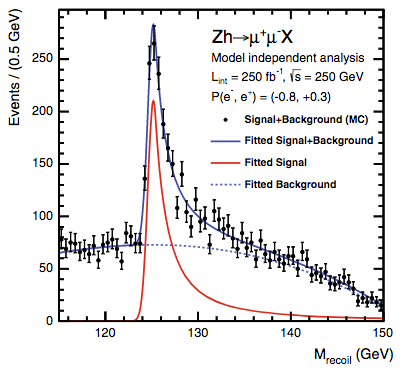
\includegraphics[width=0.5\linewidth]{chap2/fig/HiggsRecoilMuMu.png}
  \caption{The recoil mass distribution for $Zh \rightarrow \mu^+\mu^-X$ at $\sqrt{s}$ = 250 GeV for 250 fb$^{-1}$ integrated luminosity and beam polarisation of (+80\%, -30\%). Simulated with $m_h$ = 125 GeV. Taken from \cite{Thomson2016}} \label{fig:HiggsRecoilMuMu}
\end{figure}

Fits to signal and background are used to extract $m_h$. One can observe a tail to higher reconstructed recoil masses which is coming from events in which initial state radiation (\acrshort{isr}) modified the four-momentum of the collision. However, this can be accounted for during the reconstruction without shifting systematically the extracted Higgs mass. Combining the two lepton channels, a statistical precision of 32 MeV on the Higgs mass can be achieved, resulting in an uncertainty of 2.5\% on the production cross-section.

\subsubsection{Higgs BR and couplings}

Deviations from the SM Higgs couplings are in the order of less than 1\% in many new physics models beyond the SM. This requires a very high precision measurement of the Higgs coupling strength to the SM particles. At the ILC, the full Higgsstrahlung inclusive production cross-section is proportional to the square of the coupling between the Z and Higgs, $g_{hZZ}$
\begin{equation}
  \sigma(e+e- \rightarrow Zh) \propto g^2_{hZZ}
\end{equation}
The branching ratio of a decay channel is expressed as
\begin{equation}
  BR(h \rightarrow XX) = \frac{\Gamma(h \rightarrow XX)}{\Gamma_{h}}
\end{equation}
where $\Gamma_{h}$ is the full decay width of the Higgs and $\Gamma(h \rightarrow XX)$, the partial decay width with $\Gamma(h \rightarrow XX) \propto g^2_{hXX}$. Typically in a collider, quantity measured is the event rate of a certain final state corresponding to the product of the production cross-section and BR. Thus the final state cross-section at the ILC for the Higgsstrahlung and VBF production is expressed as
\begin{equation}
  \begin{aligned}
    &\sigma(e+e- \rightarrow Zh) \times BR(h \rightarrow XX) \propto \frac{g^2_{hZZ} \times g^2_{hXX}}{\Gamma_{h}}\\
    &\sigma(e+e- \rightarrow h\nu_e\nu_e) \times BR(h \rightarrow XX) \propto \frac{g^2_{hWW} \times g^2_{hXX}}{\Gamma_{h}}
  \end{aligned}
\end{equation}
By measuring the inclusive cross-section $\sigma(e+e- \rightarrow Zh)$ with the recoil technique above, a direct measure of $g_{hZZ}$ is done. A precision of 1.3\% can be achieved for this coupling for 250 fb$^{-1}$ integrated luminosity. The ratio of $\sigma(e+e- \rightarrow Zh)$ and $\sigma(e+e- \rightarrow h\nu_e\nu_e)$ for the same final state of the Higgs (e.g. $h \rightarrow bb$) yields the coupling $g_{hWW}$.

Thus it is only needed to measure the branching ratio $BR(h \rightarrow WW^*)$ to calculate $\Gamma_{h}$. The measurement of $\sigma(e+e- \rightarrow Zh) \times BR(h \rightarrow WW^*)$ and/or $\sigma(e+e- \rightarrow h\nu_e\nu_e) \times BR(h \rightarrow WW^*)$ provide the determination of $\Gamma_{h}$.
\begin{figure}[htbp!]
  \centering
  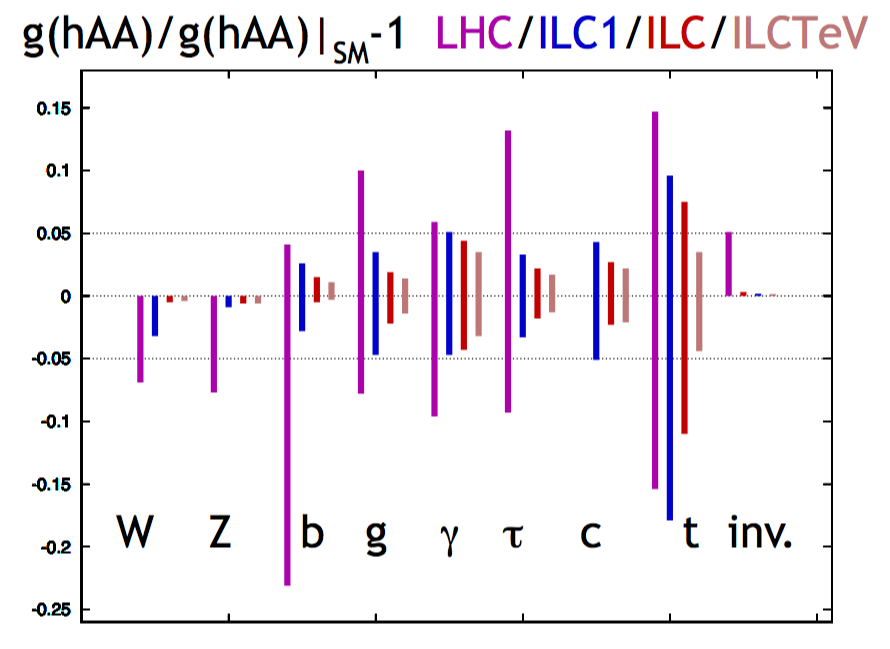
\includegraphics[width=0.6\linewidth]{chap2/fig/HiggsCouplings.png}
  \caption{Relative precision to the Higgs couplings in a model-independent way. 1 $\sigma$ confidence intervals is shown. The four sets are LHC with 300 fb$^{-1}$, 250 fb$^{-1}$ at 250 GeV, 500 fb$^{-1}$ at 500 GeV and the 1 TeV ILC program.}  \label{fig:HiggsCouplings}
\end{figure}

All inclusive cross-section measurements will be included into a global fit to minimize the uncertainty on $\Gamma_{h}$. The figure \ref{fig:HiggsCouplings} shows the relative precision achievable for the ILC compared to the LHC. In most of the measurements, the ILC is one order of magnitude more precise.

\subsubsection{Higgs self-coupling}

The triple Higgs coupling $\lambda$ can be studied at the ILC via the Higgsstrahlung or VBF production starting at around $\sqrt{s}$ = 350 GeV. The cross-section maximizes at around $\sqrt{s}$ = 500 GeV dominated by the Higgsstrahlung production. A study \cite{Duerig:2016dvi} has found that an excess of 3.5$\sigma$ can be detected and the cross-section can be measured to a 30\% precision for 2 ab$^{-1}$ integrated luminosity and a beam polarisation of (-80\%, +30\%). Due to the contribution of irreducible background diagrams without self-coupling, this results in a precision of 49\% on the Higgs self-coupling $\lambda$. At 1 TeV, the measurement of $\lambda$ in the WW channel is opened and leads to a precision of 16\% on $\lambda$ due to a smaller contribution of background diagrams.

\subsection{Electroweak Physics}

The ILC gives access to an unprecedented level of precision for the measurement of W and Z masses, widths and couplings. The production processes $e^+e^- \rightarrow W^+W^-$, $e^+e^- \rightarrow ZZ$, $\gamma\gamma \rightarrow W^+W^-$ and triple boson production $e^+e^- \rightarrow VVV$ can be studied. Additionally, vector boson scattering can be studied at high energies to constrain furthermore the Electroweak (EW) sector and search for deviations in the structure of the EW sector of the SM. Many new physics models beyond the SM predict new couplings to the W and Z bosons, thus mixing effects of the new bosons could be detected by the ILC precision measurements.

\subsection{Top mass measurement}

The top quark is the heaviest particle in the Standard Model with a mass of 173 GeV, implying that it is the most strongly coupled particle to the Higgs. The top quark is expected to be one of the most promising windows to new physics beyond the SM at the TeV energy scale. The top quark was discovered at the Tevatron by the D0 and CDF experiments \cite{Abe:1995hr, D0:1995jca}, and has only been studied by hadron colliders so far. The ILC would be the first machine to study the top quark using a leptonic initial state.

The top quark has a very short lifetime ($10^{-25}$ s), the top quark decays before hadronization thus the top quark is a "bare" quark. It decays almost to only $t \rightarrow W^+b$ were the b quark is almost only left-handed polarized. At the ILC, the top quark mass can be measured at the threshold of $\sqrt{s} \sim 2 m_t$ as the machine can be tuned in energy. Thus the shape of the top cross-section production can be measured allowing precise measurement of the top mass $m_t$, width $\Gamma_t$ and strong coupling $\alpha_s$. Additionally, the initial polarization state can be tuned to enhance the cross-section. Via this method, the top mass can be measured to a statistical precision of around 30 MeV but the final mass is mostly dominated by theoretical uncertainties of around 100-200 MeV. However, to achieve such precision, it is required to have a b-tagging efficiency and purity better than 90\% and jet energy resolution below 4\%. These requirements are met by the ILC detectors.

\subsection{Beyond the Standard Model}

The Standard Model is so far the most accurate model that describes our universe. But it has still deficiencies in some places such as the origin of mass, the strong CP problem, neutrino masses, matter-antimatter asymmetry, dark matter, gravity and more. Various theories are being developed by theorist to try to answer these questions. One of these theories is Supersymmetry (SUSY). The ILC has the potential to offer high precision measurement studies of any new particles that could be produced, but unfortunately not discoverable due to the high QCD background at the LHC. So far, LHC searches provide limits on the new particles and push the SUSY models towards naturalness with a low value of $M_{\mu} \sim M_Z$. This leads to a particle spectrum of several light super-particles charginos and neutralinos, around 150 GeV in mass, which are mass-degenerated (10-20 GeV mass gap). This would be nearly impossible to detect at the LHC. However, the ILC would have access to this new array of particles.
